\cleardoublepage

\chapter{Resultados}
\label{resultados}

En este capítulo discutiremos los resultados obtenidos a lo largo de los diferentes experimentos realizados, utilizando para ello las imágenes del conjunto de validación.
\medskip

Comenzaremos evaluando los resultados obtenidos con el algoritmo de \textit{Policy Gradient}. Podemos observar en la figura \ref{fig-resultados-experimentos-policy-gradient} que los resultados fueron en general satisfactorios con lo que buscábamos en un principio y en general el entrenamiento se mantuvo particularmente estable con respecto a los demás experimentos.
\medskip

Sin embargo, en algunas ocasiones se aprecia que si el sujeto se encuentra en un extremo de la imagen, el agente no es capaz de moverse con soltura hacia ese lado tal y como vemos en la figura \ref{fig-resultados-experimentos-policy-gradient} (b) y (c).
\medskip

Por lo general podemos decir que el agente se comporta de manera correcta, pero el número de acciones y su rendimiento en imágenes que podemos denominar extremas, todavía tiene un margen considerable de mejora.
\medskip

\begin{figure}[H]
    \centering
	\subfloat[4 acciones tomadas]{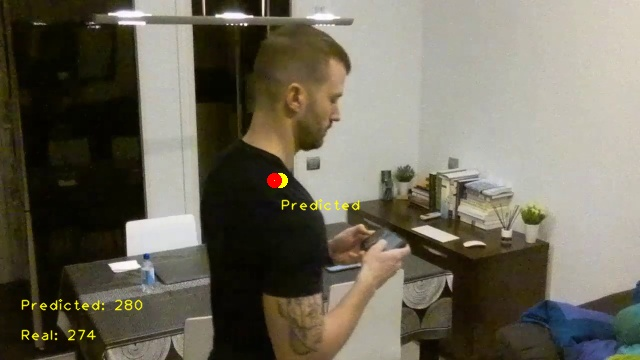
\includegraphics[width = 0.4\linewidth]{figuras/experiments/policy_gradient/test_images/33_real_274_predicted_280_actions_taken_4_pg_50epochs.jpg}}
	\hspace{0.05\linewidth}
	\subfloat[9 acciones tomadas]{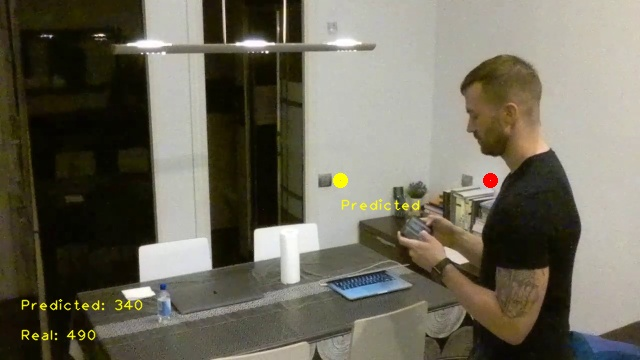
\includegraphics[width = 0.4\linewidth]{figuras/experiments/policy_gradient/test_images/34_real_490_predicted_340_actions_taken_9_pg_50epochs.jpg}}
	\hspace{0.05\linewidth}
	\subfloat[5 acciones tomadas]{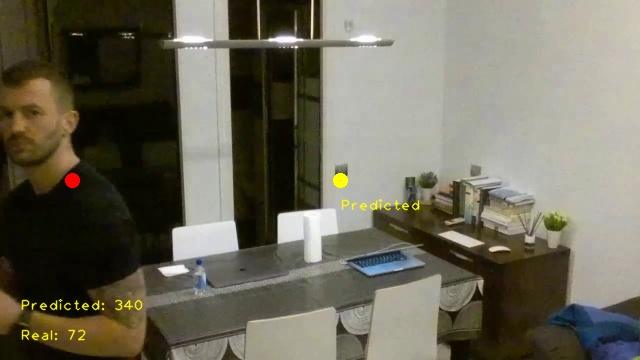
\includegraphics[width = 0.4\linewidth]{figuras/experiments/policy_gradient/test_images/53_real_72_predicted_340_actions_taken_5_pg_50epochs.jpg}}
	\hspace{0.05\linewidth}
	\subfloat[7 acciones tomadas]{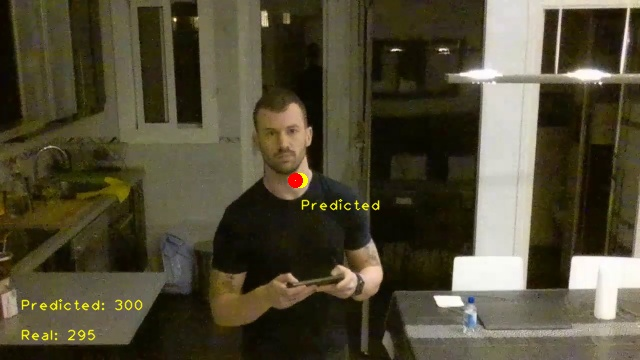
\includegraphics[width = 0.4\linewidth]{figuras/experiments/policy_gradient/test_images/87_real_295_predicted_300_actions_taken_7_pg_50epochs.jpg}}
    % \caption[Así aparece el rótulo en el índice]{Así aparece el rótulo en el texto.}
    \caption[Imágenes obtenidas en los experimentos usando \textit{Policy Gradient}]{Imágenes obtenidas en los experimentos usando \textit{Policy Gradient} sobre el conjunto de test.}
    \label{fig-resultados-experimentos-policy-gradient}
\end{figure}

A continuación analizaremos los resultados obtenidos con el algoritmo \textit{Actor Critic}. En la figura \ref{fig-resultados-experimentos-actor-critic-no-movement} vemos un ejemplo del comportamiento que comentamos durante el análisis en la sección anterior y es que el agente decide no moverse al principio del entrenamiento.
\medskip

En las 4 imágenes presentadas el agente decidió no tomar ninguna acción sino directamente permanecer quieto y con ello terminar el episodio.
\medskip

\begin{figure}[ht!]
    \centering
	\subfloat[]{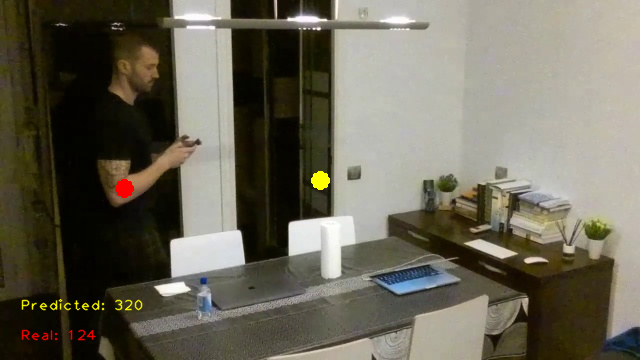
\includegraphics[width = 0.4\linewidth]{figuras/experiments/actor_critic/results/no_movement/image_11_actions_taken_0_reward_0.71875.png}}
	\hspace{0.05\linewidth}
	\subfloat[]{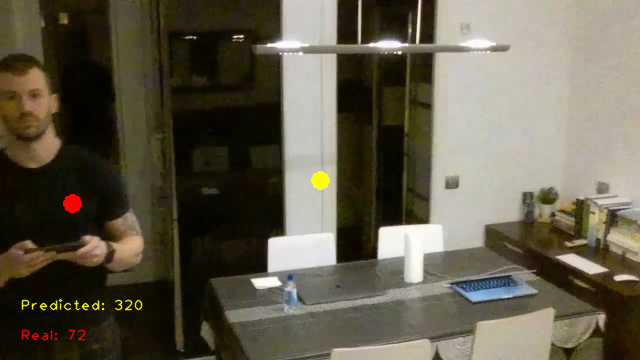
\includegraphics[width = 0.4\linewidth]{figuras/experiments/actor_critic/results/no_movement/image_12_actions_taken_0_reward_0.625.png}}
	\hspace{0.05\linewidth}
	\subfloat[]{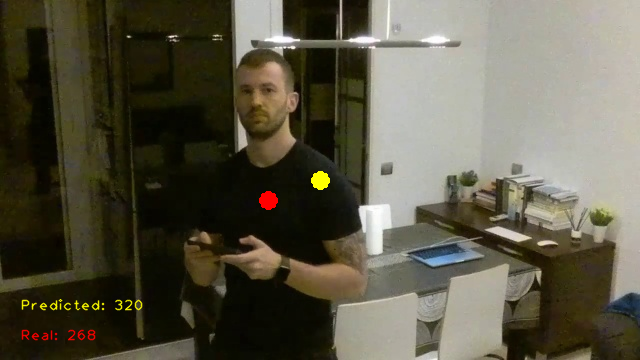
\includegraphics[width = 0.4\linewidth]{figuras/experiments/actor_critic/results/no_movement/image_13_actions_taken_0_reward_0.9375.png}}
	\hspace{0.05\linewidth}
	\subfloat[]{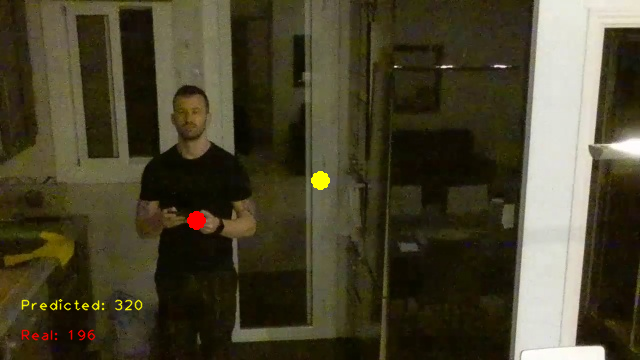
\includegraphics[width = 0.4\linewidth]{figuras/experiments/actor_critic/results/no_movement/image_14_actions_taken_0_reward_0.8125.png}}
    % \caption[Así aparece el rótulo en el índice]{Así aparece el rótulo en el texto.}
    \caption[Imágenes obtenidas con \textit{Actor Critic} sin incentivar al agente a moverse]{Imágenes obtenidas con \textit{Actor Critic} sin incentivar al agente a moverse.}
    \label{fig-resultados-experimentos-actor-critic-no-movement}
\end{figure}

La dificultad de diagnosticar este problema fue que, siguiendo las gráficas del entrenamiento, el agente parecía estar teniendo una muy buena \textit{performance} para el conjunto de entrenamiento y de test y era dificil descubrir que decidia no moverse hasta que hicimos un registro de las acciones tomadas por este en cada etapa del entrenamiento.
\medskip

\begin{table}[H]
\centering
\resizebox{\textwidth}{!}{
\begin{tabular}{@{}ccc@{}}
\toprule
\textbf{Época} & \textbf{Recompensa media} & \textbf{Número de acciones tomadas}\\ \midrule
2             & 0.8755                  & 0.366                                                     \\ \midrule
4             & 0.873                  & 0.088                                                    \\ \midrule
6             & 0.872                  & 0.071                                                   \\ \midrule
10             & 0.873                  & 0.059                                                   \\ \midrule
20             & 0.874                  & 0.053                                                   \\ \bottomrule
\end{tabular}
}
% \caption[Así aparece el rótulo en el índice]{Así aparece el rótulo en el texto.}
\caption[Resultados Actor Critic - Media de acciones tomadas por el agente en el conjunto de test]{Resultados Actor Critic - Media de acciones tomadas por el agente en el conjunto de test}
\label{table-resultados-actor-critic-numero-movimientos-imagenes-test}
\end{table}


La tabla \ref{table-resultados-actor-critic-numero-movimientos-imagenes-test} muestra un ejemplo de la evolución de la media de acciones tomadas por el agente sobre el conjunto de test en las diferentes etapas del entrenamiento.
\medskip

Cabe destacar que este patrón se produjo desde los primeros experimentos con \textit{Actor Critic}, y que como vemos en la anterior tabla, la recompensa media no baja significativamente, mientras que el número de acciones media si lo hace. Lo cual también nos hizo recapacitar en cuanto a las diferentes opciones de recompensa de nuestro agente tal y como comentamos en el capítulo previo.
\medskip

También pudimos apreciar que el rendimiento del agente por lo general disminuia según avanzaba el entrenamiento y al mismo tiempo la duración de los episodios aumentaba, por lo que se producía un punto de inflexión el cual no pudimos explicar. La figura \ref{fig-resultados-experimentos-actor-critic-same-image} muestra un ejemplo de esta evolución del agente durante el entrenamiento.
\medskip

\begin{figure}[H]
    \centering
	\subfloat[Epoch 6 - 1 acción tomada, recompensa 0.9375]{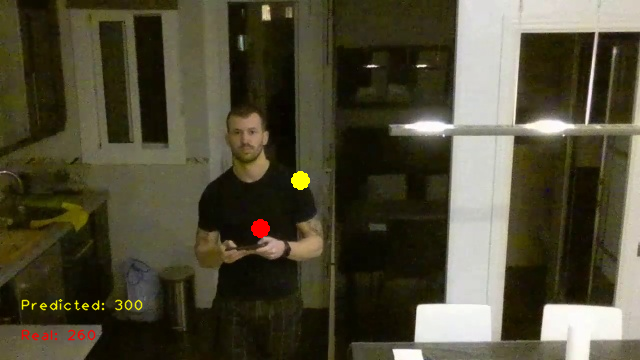
\includegraphics[width = 0.4\linewidth]{figuras/experiments/actor_critic/results/same_image_different_epochs/epoch_6_image_21_actions_taken_1_reward_0.9375.png}}
	\hspace{0.05\linewidth}
	\subfloat[Epoch 10 - 2 acciones tomadas, recompensa 0.96875]{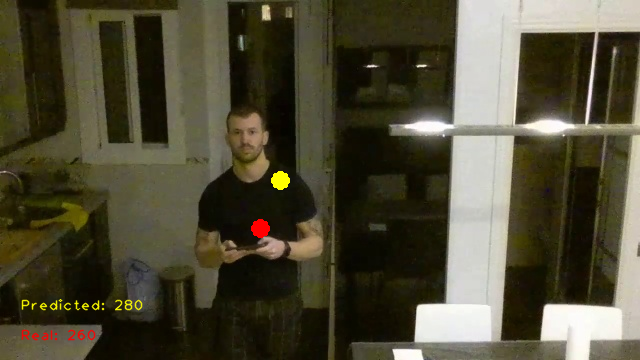
\includegraphics[width = 0.4\linewidth]{figuras/experiments/actor_critic/results/same_image_different_epochs/epoch_10_image_21_actions_taken_2_reward_0.96875.png}}
	\hspace{0.05\linewidth}
	\subfloat[Epoch 14 - 3 acciones tomadas, recompensa 0.875]{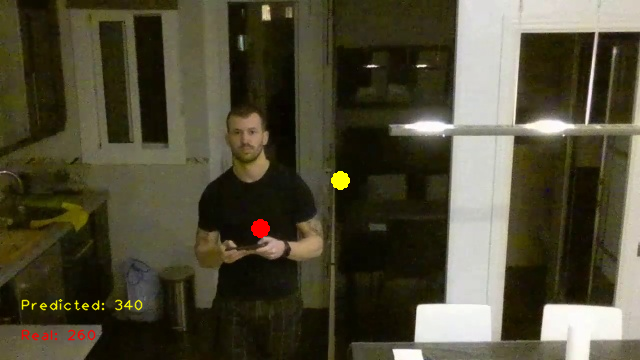
\includegraphics[width = 0.4\linewidth]{figuras/experiments/actor_critic/results/same_image_different_epochs/epoch_14_image_21_actions_taken_3_reward_0.875.png}}
	\hspace{0.05\linewidth}
	\subfloat[Epoch 20 - 4 acciones tomadas, recompensa 0.84375]{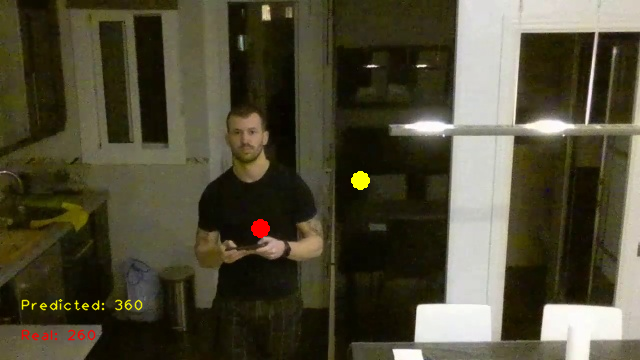
\includegraphics[width = 0.4\linewidth]{figuras/experiments/actor_critic/results/same_image_different_epochs/epoch_20_image_21_actions_taken_4_reward_0.84375.png}}
    % \caption[Así aparece el rótulo en el índice]{Así aparece el rótulo en el texto.}
    \caption[Misma imagen en diferentes etapas del entrenamiento usando \textit{Actor Critic}]{Misma imagen en diferentes etapas del entrenamiento usando \textit{Actor Critic}.}
    \label{fig-resultados-experimentos-actor-critic-same-image}
\end{figure}

Alrededor de las primeras épocas es cuando nuestro algoritmo tuvo un mejor rendimiento y es en ese momento en el que podríamos decir que nuestro agente podría desplegarse en el dispositivo final ya que combina en general pocas decisiones y hacia el lugar adecuado.
\medskip

Para finalizar el análisis de los diferentes experimentos, podemos comentar que nuestro experimento que incluyó el uso de \textit{Vision Transformers} no obtuvo ninguna ventaja con respecto a los anteriores, aunque esto también puede deberse a la calidad y cantidad de nuestros datos y al hecho de que el tiempo de entrenamiento no fue lo suficiente para permitir aprovechar la potencia de estas redes.
\medskip


